\section{Diskussion}
\label{sec:Diskussion}
Bereits die Bestimmung der Durchlassfrequenz ist nicht eindeutig gelungen. Das lag unter anderem daran, dass keine Verstärkung eingestellt wurde, was dazu führte dass die Werte eine
höhere Unsicherheit haben. Zudem haben der Spannungsgenerator, der eine Sinusspannung erzeugte, und das Millivoltmeter erheblich in den Werten geschwankt. Wenn auf dem Spannungsgenerator an dem Frequenzregler gedreht wurde, 
konnte keine bestimmte Frequenz eingestellt werden, weil die ausgegebene Frequenz nie eindeutig war. Stattdessen oszilierte sie um $\SI{5}{\kilo\hertz}$.
Aber auch das Millivoltmeter schwankte, wenn sich an dem Millivoltmeter dann doch ein Wert klar eingestellt hatte. Dies führte dazu, dass nicht nur sehr ungenaue, sondern auch sehr wenig Messwerte aufgenommen wurden.
Es wurde versucht das auszumessende Spektrum von $\SIrange{20}{40}{\kilo\hertz}$ in jeweils $\SI{2}{\kilo\hertz}$ Schritten durchzugehen und dann um das gemessene Maximum nähere Werte zu vernehmen.
Es musste dabei allerdings mehrere Male die Skalierung des Millivoltmeters geändert werden, was dazu führte, dass sich die Messwerte um ganze Faktoren verändert haben. 
So ist in \autoref{fig:daten1} zu erkennen, dass sich bei einer Reskalierung die Spannung von $\SI{5,325}{\volt}$ in der Spanne von $\SI{1}{\kilo\hertz}$ auf $\SI{24}{\volt}$ erhöhte.
Wegen dieser hohen Differenz wurde nicht nur dieser, sondern auch die anderen beiden rot markierten Werte aus den Messungen herausgenommen. 
In der folgenden \autoref{tab:finale} sind die experimentell bestimmten magnetischen Suszeptibilitäten für Neodym, Gadolinium und Dysprosium, ihre theoretischen Werte und die Abweichung der bestimmten Werten zu den Theoriewerten zu entnehmen.
\begin{table}[H]
    \centering
    \caption{Experimentell und theoretisch bestimmte Werte für die magnetische Suszeptibilität.}
    \label{tab:finale}
    \begin{tabular}{c| c c c}
        \toprule
        Stoff & Theoriewert $\chi \cdot 10^{-3} $ & $\chi_1$ & $\chi_2  \cdot 10^{-3}$ \\
        \midrule
        Neodym & 2,998 & $1,956 \pm 0$ & $3,76 \pm 0,21$ \\
        Gadolinium & 13,689 & $1,679 \pm 0,023$ & $10,70 \pm 0,6$ \\
        Dysprosium & 20,329 &$0,743 \pm 0$ & $20,30 \pm 0$ \\
      \bottomrule
    \end{tabular}
\end{table}

\noindent
Damit folgen die Abweichungen, abzulesen aus \autoref{tab:abweichung}.
\begin{table}[H]
    \centering
    \caption{Experimentell und theoretisch bestimmte Werte für die magnetische Suszeptibilität.}
    \label{tab:abweichung}
    \begin{tabular}{c| c c}
        \toprule
        Stoff & Abweichung von $\chi_1$ & Abweichung von $\chi_2$ \\
        \midrule
        Neodym &  $95,64 \pm 0,0 \%$ & $26,00 \pm 0,07 \%$ \\
        Gadolinium & $67,9 \pm 2,3 \%$ & $22,00 \pm 0.04 \%$ \\
        Dysprosium & $25,72 \pm 0,0\%$ & $3,80 \pm 0 \%$ \\
      \bottomrule
    \end{tabular}
\end{table}


\noindent
Dabei ist zu vermerken, dass die Abweichungen für die Werte von $\chi_1$ im Rahmen der oben genannten Probleme noch recht gut ist. Jedoch sind die Unsicherheiten von $\chi_2$ zu hoch um qualitative Aussagen treffen zu können.
Gerade bei der zweiten Methode zur Berechnung der magnetischen Suszeptibilität ist es besonders wichtig genau Messwerte zu messen, da hier der Unterschied zweier gemessener Widerstände für die Berechnung benötigt wird. So musste bei dieser Methode
die Brückenspannung möglichst nahe der null sein. Es war allerdings nur möglich die Werte der Spannung auf $\SI{60}{\milli\volt}$, beziehungsweise nach erneuter Skalierung des Millivoltmeters auf
$\SI{13,5}{\milli\volt}$ zu senken. Es hat hier aber auch nichts geändert, ob die Verstärkung auf 100 oder auf null lag.
Da die Brückenschaltung in einem Kasten verborgen ist, kann keine Aussage darüber getroffen werden, ob vielleicht hier noch mögliche Quellen der Unsicherheit sind.


\section{Anhang}
\label{sec:Anhang}

\begin{figure}[H]
    \centering
    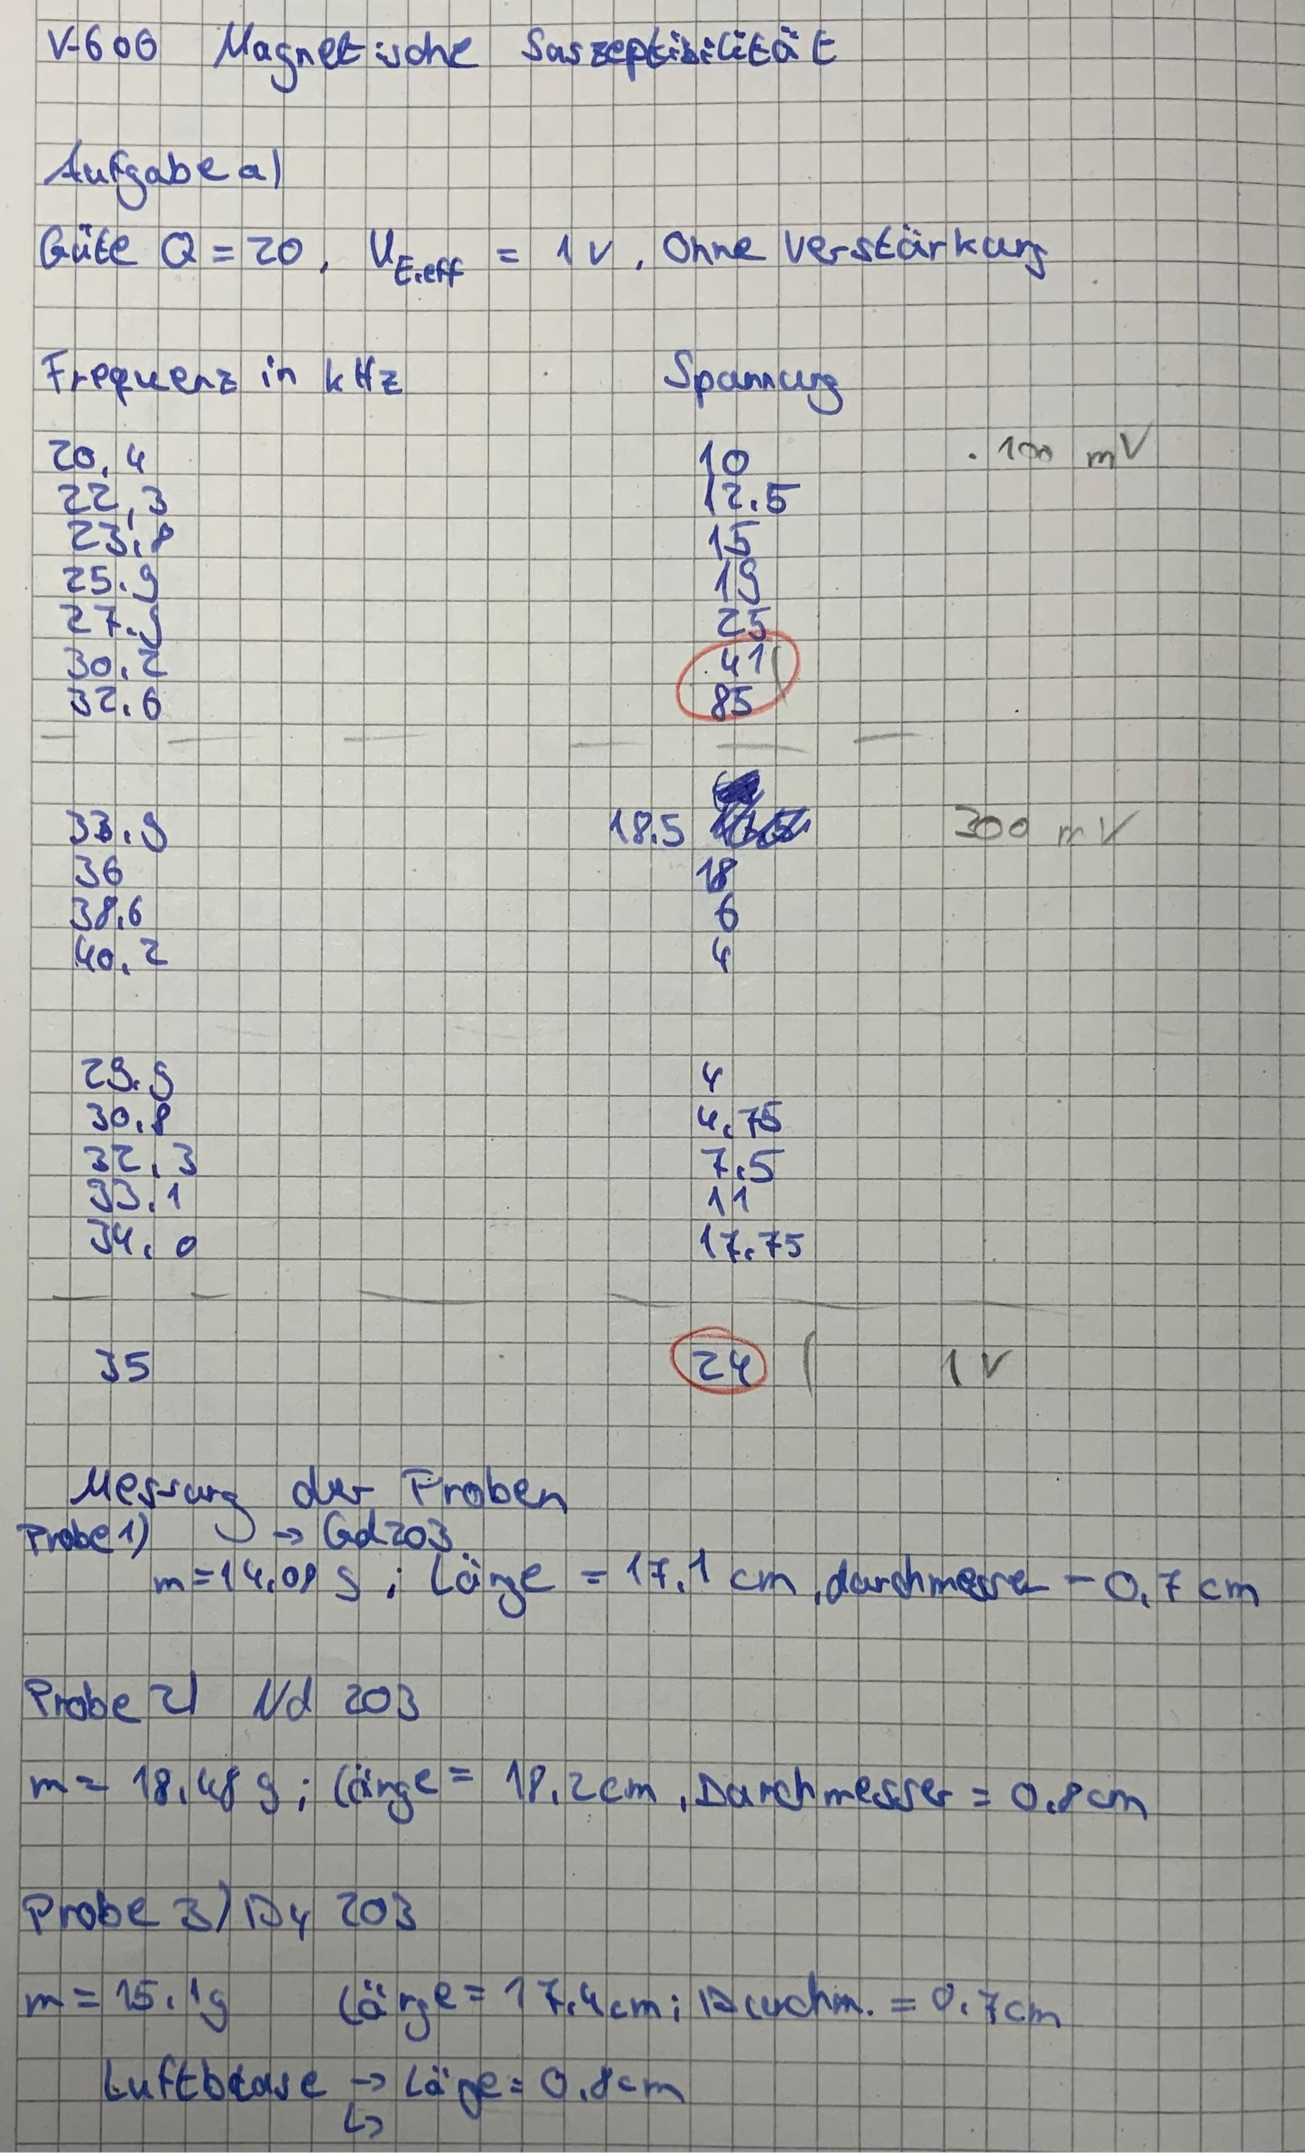
\includegraphics[width=0.75\textwidth]{data/origDaten1.jpg}
    \caption{Originale Messdaten.}
    \label{fig:daten1}
\end{figure}

\begin{figure}[H]
    \centering
    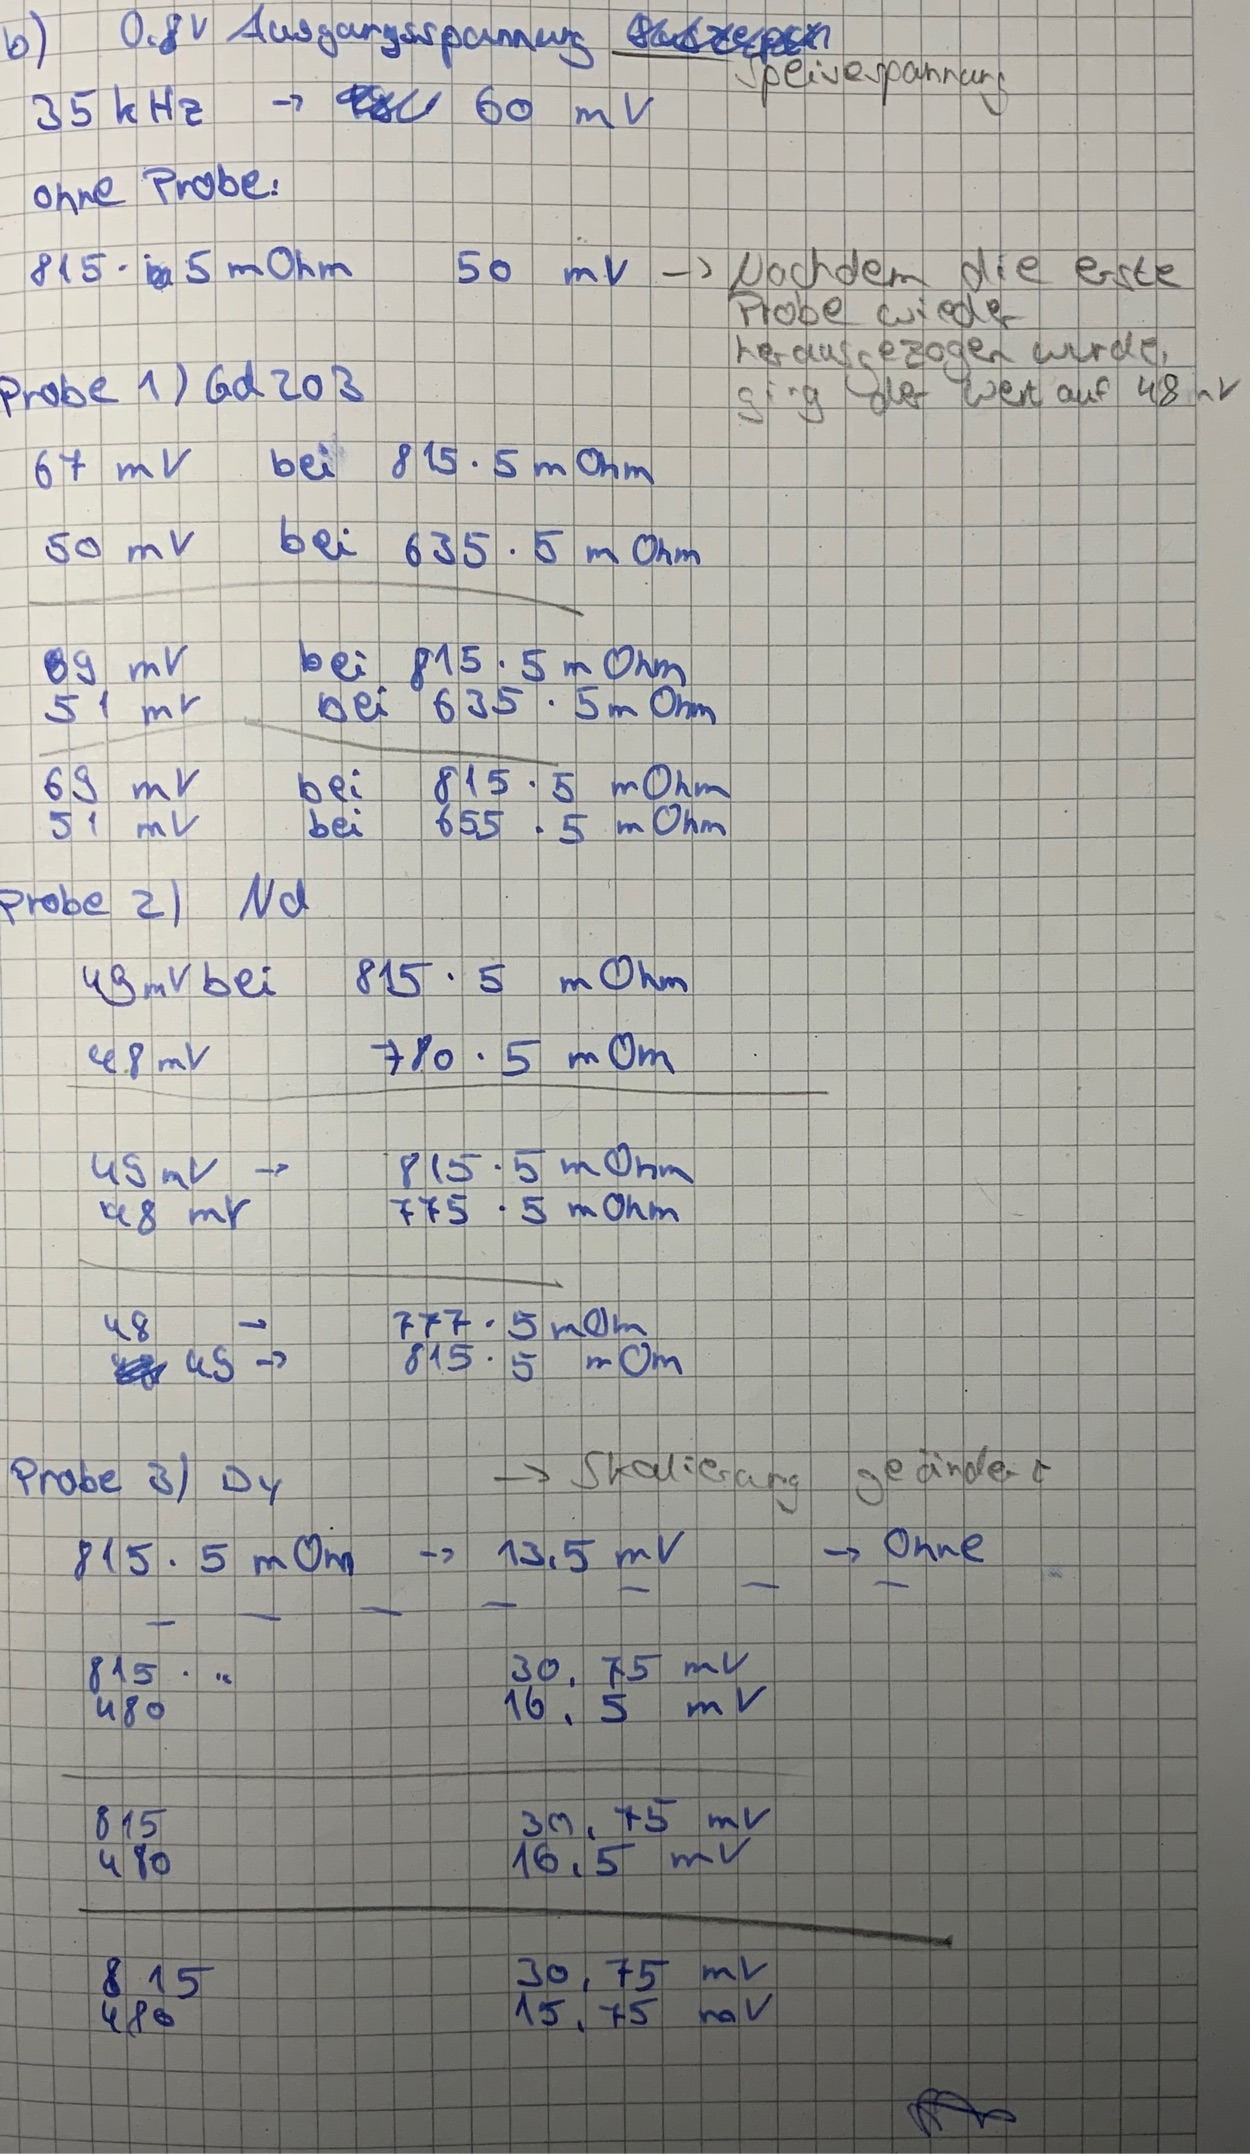
\includegraphics[width=0.75\textwidth]{data/origDaten2.jpg}
    \caption{Originale Messdaten.}
    \label{fig:daten2}
\end{figure}